\documentclass[12pt,a4paper]{report}

% Kodowanie i język
\usepackage[utf8]{inputenc}
\usepackage[T1]{fontenc}
\usepackage[polish]{babel}
\usepackage{lmodern}

% Marginesy
\usepackage[margin=2.5cm]{geometry}

% Grafika i kolory
\usepackage{graphicx}
\usepackage{xcolor}

% Tabele
\usepackage{booktabs}
\usepackage{longtable}
\usepackage{tabularx}
\usepackage{array}
\usepackage{multirow}

% Listy
\usepackage{enumitem}

% Kod źródłowy
\usepackage{listings}
\usepackage{lstautogobble}

% Hiperłącza
\usepackage[hidelinks,colorlinks=false]{hyperref}

% Nagłówki i stopki
\usepackage{fancyhdr}

% Interlinea
\usepackage{setspace}
\onehalfspacing

% Wcięcia
\usepackage{parskip}
\setlength{\parskip}{0.5em}

% Definicja koloru dla kodu
\definecolor{codeblue}{RGB}{0,102,204}
\definecolor{codegray}{RGB}{128,128,128}
\definecolor{codegreen}{RGB}{0,128,0}
\definecolor{codebg}{RGB}{248,248,248}
\definecolor{codeborder}{RGB}{220,220,220}

% Styl dla kodu
\lstdefinestyle{mystyle}{
    backgroundcolor=\color{codebg},
    commentstyle=\color{codegreen},
    keywordstyle=\color{codeblue}\bfseries,
    numberstyle=\tiny\color{codegray},
    stringstyle=\color{codegreen!60!black},
    basicstyle=\ttfamily\small,
    breakatwhitespace=false,
    breaklines=true,
    captionpos=b,
    keepspaces=true,
    numbers=left,
    numbersep=8pt,
    showspaces=false,
    showstringspaces=false,
    showtabs=false,
    tabsize=2,
    frame=single,
    rulecolor=\color{codeborder},
    autogobble=true
}
\lstset{style=mystyle}

% Styl PHP
\lstdefinelanguage{PHP}{
    morekeywords={class,function,public,private,protected,static,return,if,else,foreach,new,use,namespace,extends,implements,interface,abstract,final,try,catch,throw,null,true,false,array,string,int,float,bool,void,mixed},
    sensitive=true,
    morecomment=[l]{//},
    morecomment=[s]{/*}{*/},
    morestring=[b]",
    morestring=[b]',
}

% Nagłówki
\pagestyle{fancy}
\fancyhf{}
\fancyhead[L]{\small Strava Clone -- Sprawozdanie projektowe}
\fancyhead[R]{\small\thepage}
\fancyfoot[C]{}
\renewcommand{\headrulewidth}{0.4pt}

% Głębokość spisu treści
\setcounter{tocdepth}{3}
\setcounter{secnumdepth}{3}


\begin{document}

\begin{titlepage}
    \centering
    \vspace*{2cm}

    {\LARGE\bfseries Sprawozdanie z projektu programistycznego\par}
    \vspace{1.5cm}

    {\Huge\bfseries Strava Clone\par}
    \vspace{0.5cm}
    {\large Aplikacja do śledzenia aktywności fizycznych\par}

    \vspace{1cm}
    {\large\bfseries Projektowanie i Programowanie Obiektowe\par}

    \vspace{1.5cm}

    \begin{tabular}{ll}
        \textbf{Technologia backendu:}  & Laravel 12 (PHP 8.2+)       \\[4pt]
        \textbf{Technologia frontendu:} & Vue 3 + TypeScript           \\[4pt]
        \textbf{Baza danych:}           & PostgreSQL 18                \\[4pt]
        \textbf{Repozytorium:}          & github.com/Console-dungeon/ \\
                                        & strava-clone                 \\
    \end{tabular}

    \vfill

    {\large \today\par}
\end{titlepage}

\tableofcontents
\thispagestyle{empty}
\cleardoublepage


\chapter{Charakterystyka systemu}
\label{ch:charakterystyka}

\section{Cel i zakres}

Strava Clone to aplikacja webowa do rejestrowania i analizowania aktywności fizycznych. Zbudowana jest w architekturze monolitycznej z podziałem na warstwy, z użyciem frameworka \textbf{Laravel 12} na backendzie, \textbf{Vue 3 + TypeScript} na frontendzie i protokołu \textbf{Inertia.js} jako warstwy pośredniczącej.

\section{Wzorzec MVC z warstwą serwisów}

Aplikacja stosuje wzorzec Model--Widok--Kontroler rozszerzony o dedykowaną warstwę serwisów. Kontrolery delegują całą logikę biznesową do klas serwisowych (\texttt{GarminService}, \texttt{DashboardService}, \texttt{GpxParser}), pozostając cienkimi adapterami między routingiem a logiką.


\chapter{Diagramy UML}
\label{ch:diagramy}

\section{Diagram przypadków użycia (Use-Case)}

Diagram przedstawia wszystkich aktorów systemu i przypadki użycia dostępne dla każdego z nich. Wyróżniono dwa aktory: \textbf{Użytkownik} (osoba zalogowana w aplikacji) oraz \textbf{Garmin Connect} (zewnętrzny system sportowy, z którym aplikacja integruje się przez API).

\begin{figure}[h]
\centering
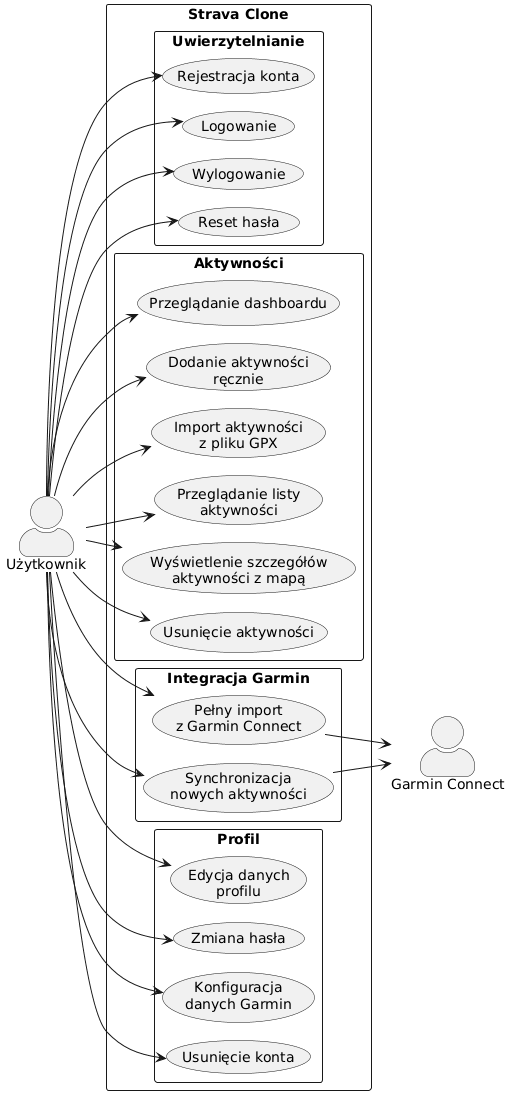
\includegraphics[width=0.95\textwidth]{usecase.png}
\caption{Diagram przypadków użycia systemu Strava Clone}
\end{figure}

\section{Diagram czynności (Activity)}

Diagram czynności ilustruje przepływ sterowania dla scenariusza dodawania aktywności przez użytkownika. Uwzględniono trzy ścieżki: ręczne wprowadzenie danych, import z pliku GPX oraz synchronizację z Garmin Connect.

\begin{figure}[h]
\centering
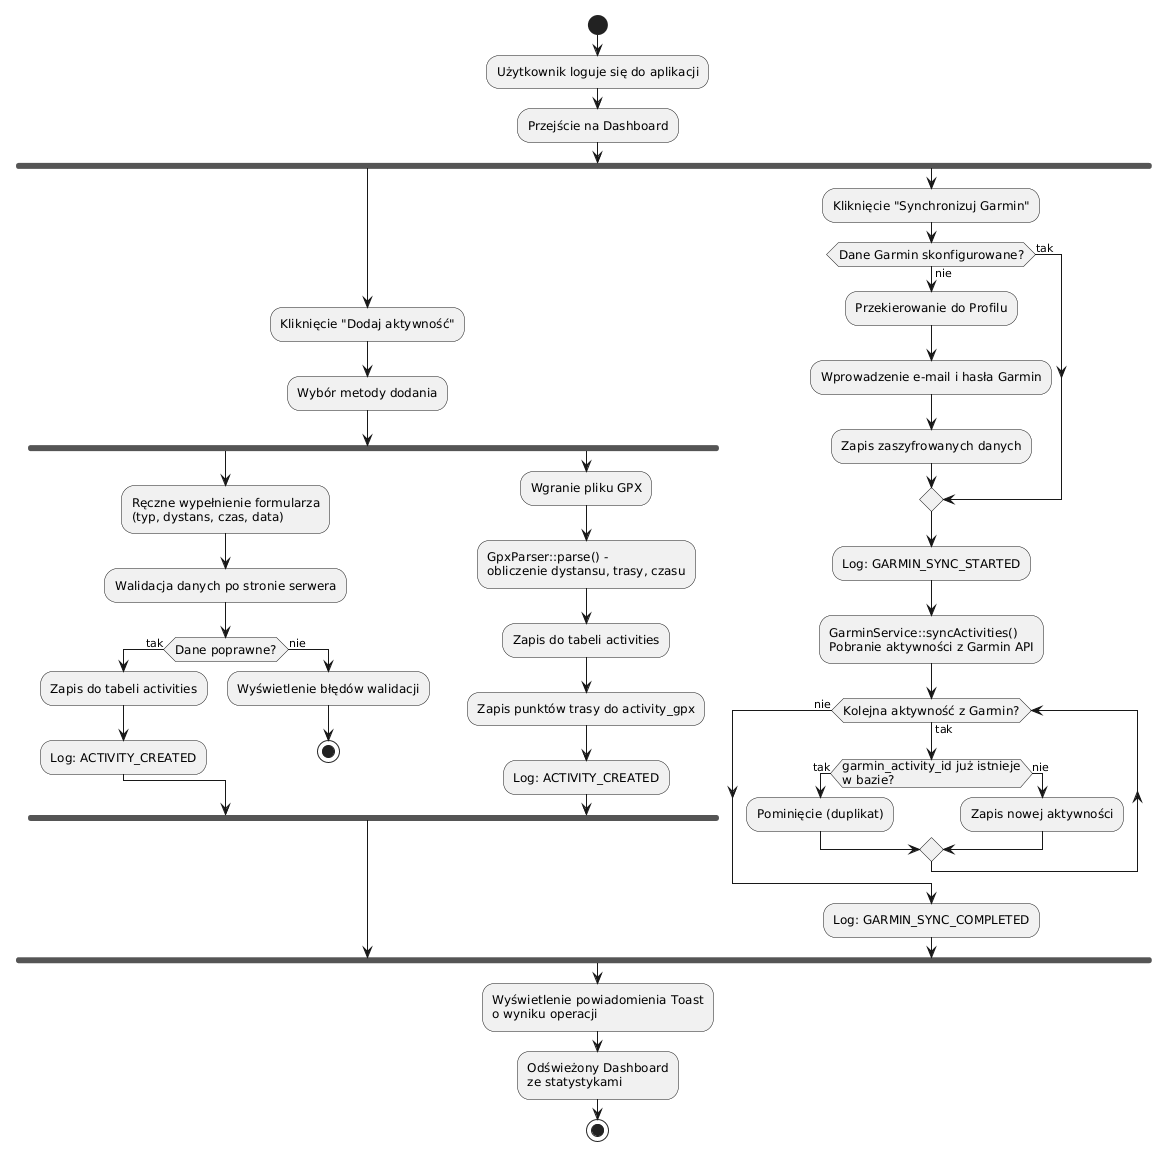
\includegraphics[width=0.95\textwidth]{activity.png}
\caption{Diagram czynności -- dodawanie aktywności i synchronizacja z Garmin}
\end{figure}

\section{Diagram klas (Class)}

Diagram klas przedstawia strukturę głównych klas systemu z podziałem na warstwy: modele Eloquent, serwisy logiki biznesowej i kontrolery. Strzałki przerywane oznaczają zależność użycia (\textit{uses}), strzałki ciągłe -- relacje między modelami (Eloquent relationships).

\begin{figure}[h]
\centering
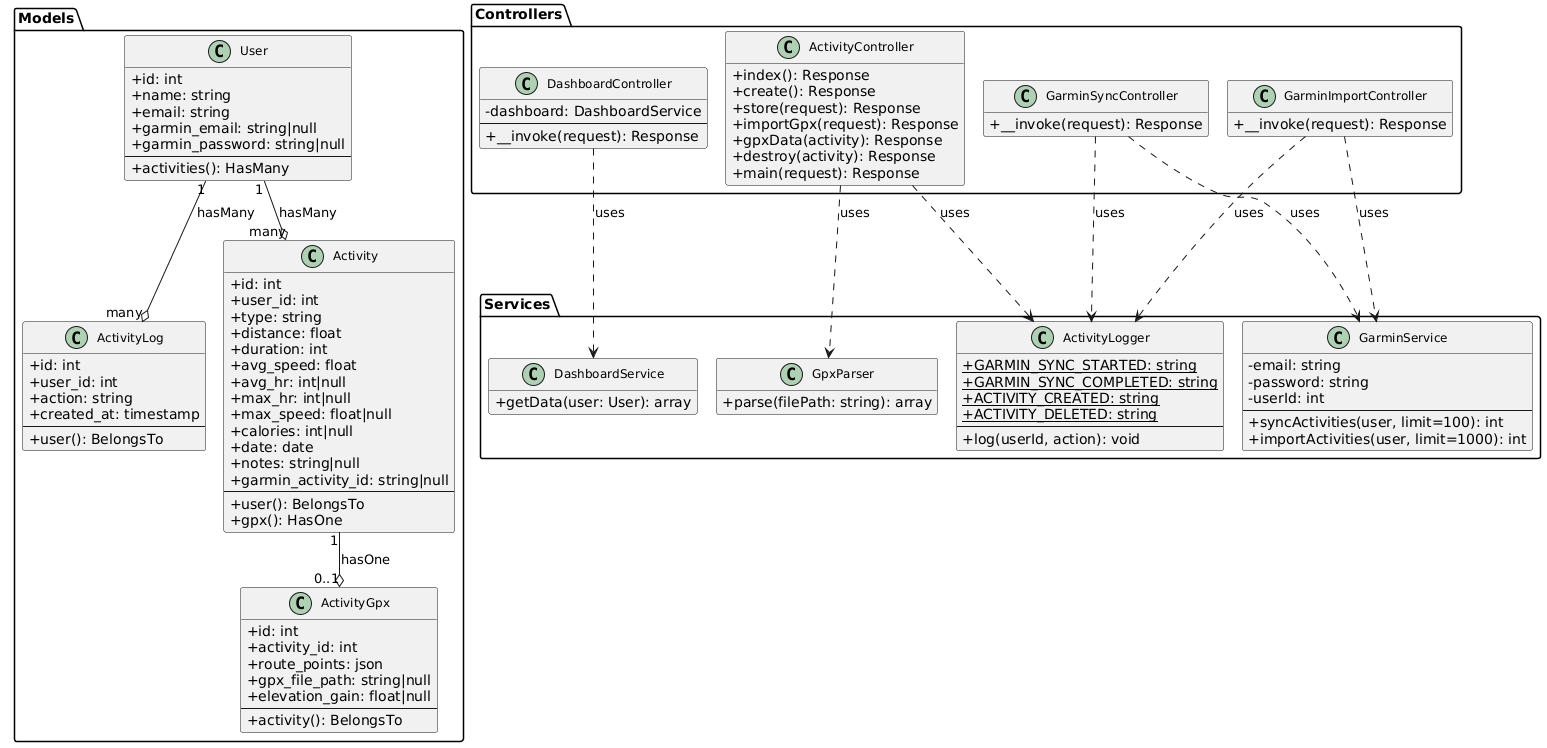
\includegraphics[width=\textwidth]{class.png}
\caption{Diagram klas -- modele, serwisy i kontrolery}
\end{figure}

\section{Diagram sekwencji (Sequence)}

Diagram sekwencji opisuje kolejność wywołań metod podczas importu aktywności z pliku GPX -- od żądania HTTP przychodzącego od użytkownika, przez parsowanie pliku, zapis do bazy danych, aż po powiadomienie zwrotne.

\begin{figure}[h]
\centering
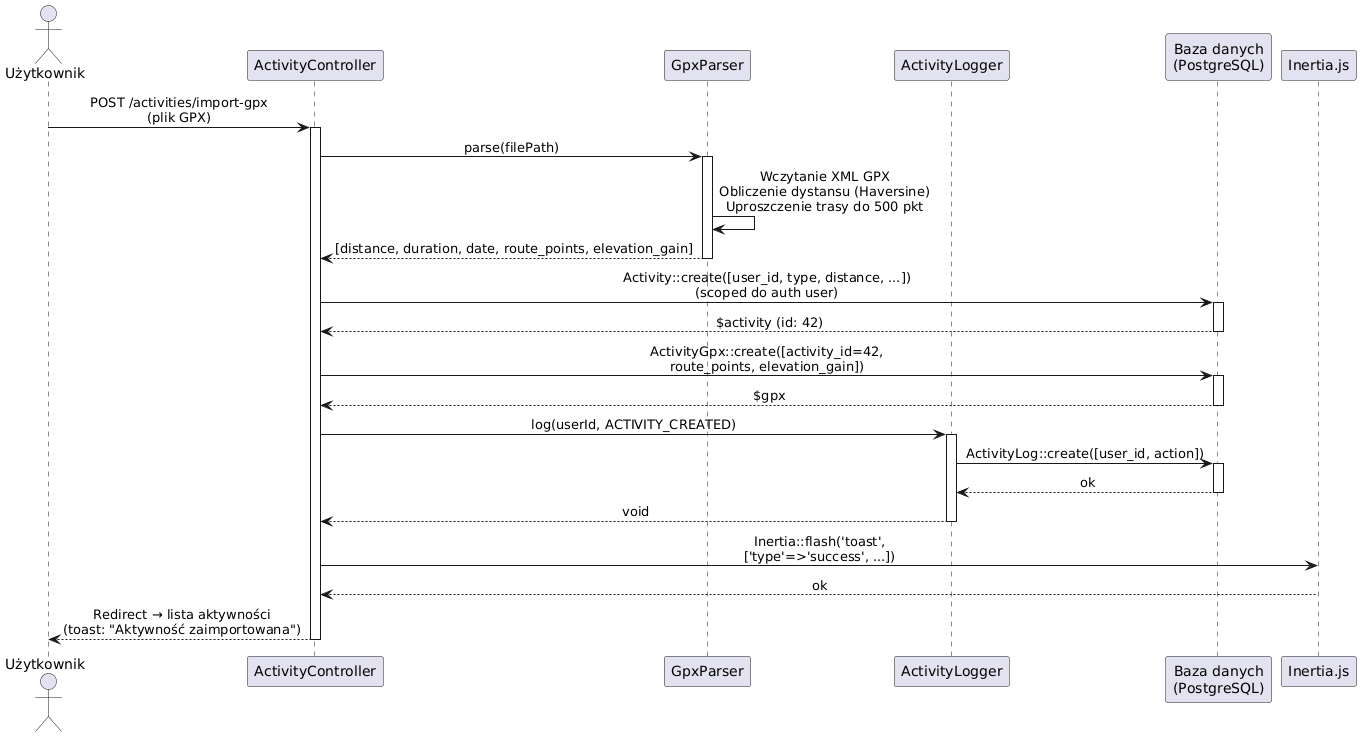
\includegraphics[width=0.95\textwidth]{sequence.png}
\caption{Diagram sekwencji -- import aktywności z pliku GPX}
\end{figure}

% ============================================================


\chapter{Opis implementacji}
\label{ch:implementacja}

\section{Wzorzec Controller--Service w praktyce}

Poniżej przedstawiono przykładową implementację kontrolera delegującego pracę do serwisu oraz przykładowy fragment serwisu obsługującego logikę biznesową.

\section{Backend}

\subsection{Laravel 12}

Framework PHP w wersji 12 dostarcza:
\begin{itemize}[noitemsep]
    \item \textbf{Routing} -- deklaratywny w \texttt{routes/web.php} i \texttt{routes/auth.php},
    \item \textbf{Eloquent ORM} -- mapowanie obiektowo-relacyjne dla PostgreSQL,
    \item \textbf{Form Requests} -- walidacja danych wejściowych w osobnych klasach,
    \item \textbf{Queue} -- asynchroniczne przetwarzanie zadań (driver: \texttt{database}),
    \item \textbf{Cache} -- buforowanie danych (driver: \texttt{database}),
    \item \textbf{Szyfrowanie} -- kolumna \texttt{garmin\_password} przechowywana zaszyfrowana (\texttt{encrypted} cast).
\end{itemize}

\subsection{Wzorzec Controller--Service}

Kontrolery są celowo cienkie: nie zawierają logiki biznesowej, jedynie delegują pracę do warstwy serwisów.

\begin{lstlisting}[language=PHP, caption=Przykładowy kontroler delegujący do serwisu]
class DashboardController extends Controller
{
    public function __construct(
        private readonly DashboardService $dashboard
    ) {}

    public function __invoke(Request $request): Response
    {
        return Inertia::render('Dashboard', [
            'data' => $this->dashboard->getData(
                auth()->guard()->user()
            ),
        ]);
    }
}
\end{lstlisting}

\subsection{Inertia.js}

Inertia.js pełni rolę warstwy pośredniczącej między backendem a frontendem. Backend nie zwraca JSON, lecz wywołuje \texttt{Inertia::render('NazwaStrony', \$props)}, co powoduje załadowanie odpowiedniego komponentu Vue z danymi jako \textit{props}. Nawigacja po aplikacji odbywa się bez przeładowania strony (SPA), przy czym serwer zawsze kontroluje dane i routowanie.

\subsection{Kluczowe serwisy}

\subsubsection{GarminService}

Odpowiada za komunikację z Garmin Connect przez pakiet \texttt{alexoid/laravel-garmin}:
\begin{itemize}[noitemsep]
    \item \texttt{importActivities()} -- pobiera do 1000 aktywności i zapisuje je w bazie,
    \item \texttt{syncActivities()} -- pobiera wyłącznie aktywności nowsze niż ostatnia zapisana.
\end{itemize}
Prędkości z Garmin (w m/s) są przeliczane na km/h przez mnożnik $\times 3{,}6$.

\subsubsection{GpxParser}

Parsuje pliki GPX (format XML) i wyodrębnia:
\begin{itemize}[noitemsep]
    \item listę punktów trasy (szerokość/długość geograficzna, wysokość, czas),
    \item całkowity dystans -- obliczony wzorem Haversine'a,
    \item przewyższenie dodatnie (\textit{elevation gain}),
    \item czas aktywności, datę, typ.
\end{itemize}
Dla wydajności trasa jest upraszczana do maksymalnie 500 punktów.

\subsubsection{DashboardService}

Agreguje dane dla dashboardu użytkownika:
\begin{itemize}[noitemsep]
    \item łączny dystans, łączny czas, średnia prędkość,
    \item lista ostatnich aktywności,
    \item dane szeregów czasowych dla wykresu.
\end{itemize}

\subsubsection{ActivityLogger}

Rejestruje akcje użytkownika w tabeli \texttt{activity\_logs}. Zdefiniowane akcje:
\texttt{GARMIN\_SYNC\_STARTED}, \texttt{GARMIN\_SYNC\_COMPLETED}, \texttt{ACTIVITY\_CREATED}, \texttt{ACTIVITY\_DELETED}.

\subsection{Uwierzytelnianie}

System uwierzytelniania oparty na \textbf{Laravel Breeze}:
\begin{itemize}[noitemsep]
    \item sesje przechowywane w bazie danych (tabela \texttt{sessions}),
    \item middleware \texttt{auth} chroni wszystkie trasy wymagające zalogowania,
    \item middleware \texttt{HandleInertiaRequests} eksponuje dane zalogowanego użytkownika (\texttt{auth.user}) do każdej strony Vue jako \textit{shared props}.
\end{itemize}


\chapter{Dokumentacja użytkowa}
\label{ch:uzytkownik}

\section{Opis funkcji i możliwości}

Strava Clone to aplikacja webowa do rejestrowania i analizowania aktywności fizycznych. Główne możliwości dostępne dla użytkownika:

\begin{itemize}
    \item \textbf{Rejestracja i logowanie} -- zakładanie konta, weryfikacja e-mail, reset hasła.
    \item \textbf{Dashboard} -- podgląd łącznego dystansu, czasu i średniej prędkości ze wszystkich aktywności; wykres aktywności w czasie; tabela ostatnich treningów.
    \item \textbf{Dodawanie aktywności ręcznie} -- wpisanie typu (bieg, rower, pływanie), dystansu, czasu trwania, daty i opcjonalnych notatek.
    \item \textbf{Import z pliku GPX} -- wgranie pliku trasy z zegarka lub aplikacji GPS; aplikacja automatycznie oblicza dystans, czas i przewyższenie oraz rysuje trasę na mapie.
    \item \textbf{Integracja z Garmin Connect} -- jednorazowy pełny import historii aktywności (do 1000) lub synchronizacja tylko nowych treningów.
    \item \textbf{Mapa trasy} -- interaktywna mapa z narysowaną trasą i markerami startu/mety (dla aktywności GPX i Garmin).
    \item \textbf{Filtrowanie i paginacja} -- filtrowanie listy aktywności według typu (bieg/rower/pływanie) oraz przeglądanie z podziałem na strony.
    \item \textbf{Usuwanie aktywności} -- trwałe usunięcie aktywności wraz z danymi trasy GPS.
    \item \textbf{Zarządzanie profilem} -- zmiana imienia, adresu e-mail, hasła, podpięcie konta Garmin lub usunięcie konta.
    \item \textbf{Tryb ciemny} -- automatyczne wsparcie dla jasnego i ciemnego motywu systemowego.
    \item \textbf{Język interfejsu} -- aplikacja dostępna w języku polskim i angielskim.
\end{itemize}

\section{Instrukcja obsługi}

\subsection{Rejestracja i pierwsze logowanie}

\begin{enumerate}[noitemsep]
    \item Otwórz aplikację pod adresem \texttt{http://localhost:8000}.
    \item Kliknij \textbf{Zarejestruj się} i wypełnij formularz (imię, e-mail, hasło).
    \item Potwierdź adres e-mail klikając link w otrzymanej wiadomości.
    \item Zaloguj się podając e-mail i hasło.
\end{enumerate}

\subsection{Dodawanie aktywności ręcznie}

\begin{enumerate}[noitemsep]
    \item Na dashboardzie kliknij \textbf{Dodaj aktywność}.
    \item Wybierz typ aktywności (Bieganie / Jazda na rowerze / Pływanie).
    \item Wpisz dystans (w km), czas trwania (w minutach), datę i opcjonalne notatki.
    \item Kliknij \textbf{Zapisz} -- aktywność pojawi się na liście i w statystykach dashboardu.
\end{enumerate}

\subsection{Import aktywności z pliku GPX}

\begin{enumerate}[noitemsep]
    \item Na stronie listy aktywności kliknij \textbf{Importuj GPX}.
    \item Wybierz plik \texttt{.gpx} z dysku (eksportowany z Garmina, Stravacompatible, itp.).
    \item Aplikacja automatycznie wyliczy dystans, czas i przewyższenie -- kliknij \textbf{Importuj}.
    \item Po imporcie możesz otworzyć aktywność i zobaczyć trasę na mapie.
\end{enumerate}

\subsection{Synchronizacja z Garmin Connect}

\begin{enumerate}[noitemsep]
    \item Przejdź do \textbf{Profil} i w sekcji \textit{Garmin Connect} wpisz e-mail i hasło konta Garmin. Kliknij \textbf{Zapisz}.
    \item Wróć na Dashboard.
    \item Kliknij \textbf{Importuj z Garmin} -- pobierze całą historię aktywności (do 1000).
    \item Przy kolejnych wizytach kliknij \textbf{Synchronizuj} -- pobierze tylko nowe aktywności.
\end{enumerate}

\subsection{Przeglądanie aktywności}

\begin{enumerate}[noitemsep]
    \item Przejdź do zakładki \textbf{Aktywności}.
    \item Użyj filtrów na górze listy, aby wyświetlić tylko wybrany typ (np. Bieganie).
    \item Kliknij aktywność na liście, aby zobaczyć szczegóły -- parametry i mapę trasy.
    \item Aby usunąć aktywność, kliknij ikonę kosza przy wybranym rekordzie i potwierdź.
\end{enumerate}

\section{Pytania i odpowiedzi (FAQ)}

\textbf{Q: Zapomniałem hasła. Co zrobić?} \\
A: Na stronie logowania kliknij \textit{Nie pamiętasz hasła?}, podaj adres e-mail i kliknij \textit{Wyślij link}. Otrzymasz wiadomość z linkiem do ustawienia nowego hasła. Link jest jednorazowy i wygasa po 60 minutach.

\vspace{0.5em}
\textbf{Q: Czy mogę importować aktywności zarówno z GPX, jak i z Garmin?} \\
A: Tak. Obie metody działają niezależnie. Aplikacja wykrywa duplikaty aktywności Garmin po unikalnym identyfikatorze \texttt{garmin\_activity\_id}, więc synchronizacja nie zduplikuje wcześniej zaimportowanych rekordów.

\vspace{0.5em}
\textbf{Q: Dlaczego na mapie nie widać trasy dla ręcznie dodanej aktywności?} \\
A: Mapa wyświetlana jest tylko dla aktywności, które zawierają dane GPS (zaimportowanych z pliku GPX lub z Garmin Connect). Aktywności dodane ręcznie nie posiadają punktów trasy.

\vspace{0.5em}
\textbf{Q: Czy moje hasło do Garmin Connect jest bezpieczne?} \\
A: Tak. Hasło przechowywane jest w bazie danych w formie zaszyfrowanej (algorytm AES-256 przez mechanizm \texttt{encrypted} Laravel). Klucz szyfrowania nie jest zapisany w bazie danych, lecz w zmiennej środowiskowej \texttt{APP\_KEY}.

\vspace{0.5em}
\textbf{Q: Co oznaczają jednostki w statystykach aktywności?} \\
A: Dystans podawany jest w \textbf{kilometrach}, czas w \textbf{minutach}, prędkość w \textbf{km/h}, tętno w \textbf{bpm}, kalorie w \textbf{kcal}, przewyższenie w \textbf{metrach}.

\vspace{0.5em}
\textbf{Q: Ile aktywności można zaimportować z Garmin naraz?} \\
A: Limit jednorazowego importu wynosi \textbf{1000 aktywności}. Kolejne synchronizacje pobierają wyłącznie aktywności nowsze niż ostatnia zapisana w bazie -- nie ma ograniczenia łącznej liczby rekordów.

\vspace{0.5em}
\textbf{Q: Jak usunąć konto?} \\
A: Przejdź do \textbf{Profil} $\to$ sekcja \textit{Usuń konto}. Wpisz hasło jako potwierdzenie i kliknij \textit{Usuń konto}. Operacja jest nieodwracalna -- zostaną usunięte wszystkie aktywności, dane trasy GPS i historia logów.

% ============================================================

\end{document}
